\documentclass{article}

\usepackage[final]{neurips_2019}

\usepackage[utf8]{inputenc}
\usepackage[T1]{fontenc}
\usepackage{hyperref}
\usepackage{url}
\usepackage{booktabs}
\usepackage{amsfonts}
\usepackage{nicefrac}
\usepackage{microtype}
\usepackage{sidecap}
% \usepackage[section]{placeins}
\usepackage{graphicx}
\usepackage{adjustbox}
\usepackage{xcolor}
\usepackage{lipsum}
\usepackage{amsmath}
\usepackage{tabularx}
\usepackage{longtable}
\usepackage{arydshln}
\usepackage{caption}
\usepackage{subcaption}
\usepackage[ruled]{algorithm2e}
\usepackage[left=1.5cm, right=1.5cm]{geometry}


\newcommand{\note}[1]{\textcolor{blue}{{#1}}}

\title{
  Walk Less and Only Down Smooth Valleys \\
  \vspace{0.15cm}
  \large \normalfont CS224N Default Project  % Select one and delete the other
}

\author{
  Quinn Hollister \\
  % ICME \\
  Stanford University \\
  \texttt{bh9vw@stanford.edu} \\
  % Examples of more authors
   \And
    Julian Cooper \\
  % ICME \\
  Stanford University \\
  \texttt{jelc@stanford.edu} \\
   \And
   Thomas Brink \\
  % ICME \\
  Stanford University \\
  \texttt{tbrink@stanford.edu} \\
}

\begin{document}

\maketitle
\vspace{-0.4cm}
\begin{abstract}
  Transfer learning has become a valuable tool for handling a variety of downstream NLP tasks given a single generic pre-trained model \cite{weiss2016survey}. Since most of the downstream tasks are specialized, quality training data is a scarce resource, making training large models from scratch very difficult. 
  In this project, we investigate how the performance of a pre-trained BERT encoder model changes for different downstream prediction tasks when we include (1) regularization in our fine-tuning loss function and parameter gradient step (SMART by Jiang et al. \cite{smart}), (2) multitask learning with task-specific datasets, and (3) rich relational layers that exploit similarity between tasks.
  We find that, while SMART is effective for preventing overfitting on smaller fine-tuning datasets, its value diminishes as we expose the model to larger task-specific training data. Our best results come from combining multitask learning with relational layers for related tasks. 
\end{abstract}
\vspace{-0.8cm}
% {\color{red} This template does not contain the full instruction set for this assignment; please refer back to the milestone instructions PDF.}

\section{Introduction}

With the advent of transformers and large language models, performance on various downstream NLP tasks drastically improved, leading to advances like ChatGPT \cite{openai2023gpt4}. These models have captivated the world with their ability to mirror human language, answer questions, and perform various tasks that only require abstract prompts. This explosion in ability can be explained partially by research in Multitask Learning (MTL) \cite{intro}, which allowed these models to aggregate training samples over various tasks, and to learn shared knowledge amongst them. This allowed more complex tasks -- which might have a labeled dataset of insignificant size -- to benefit from the language structure learned in richer data environments. The process of encouraging a model to utilize these different tasks effectively, and without "forgetting" previously hard-won language knowledge, is hard to get right and is the focus of this project. 

More specifically, in this research, we use pretrained embeddings from the BERT large-language model for three `fine-grained' tasks; sentence sentiment classification, paraphrase detection, and paired sentence semantic textual similarity \cite{wang2018glue}.
We first test the ability of BERT embeddings to be tuned towards sentence sentiment classification only - a single classifier. We then implement SMART, a state-of-the-art regularization method proposed by Jiang et al. \cite{smart}, which aims to tackle overfitting issues during the process of fine-tuning on small tasks using pretrained embeddings. Furthermore, we apply multitask learning approaches that learn on all of the three aforementioned tasks simultaneously \cite{intro}. In doing so, we explore various methods to balance learning across tasks while exploiting as much of the available data at hand \cite{MTL}. Our findings suggest that, for low-data fine-tuning tasks, SMART significantly improves performance of multitask models. This improvement vanishes when we adapt our multitask models to handle richer data during fine-tuning. In addition, we find that by sharing neural network layers across similar tasks, we can drastically improve prediction performance.

This paper continues with a short review of related work in Section \ref{sec: related-work}. Then, we discuss our model approaches in Section \ref{sec: approach}, after which we outline our main experiments and corresponding results in Section \ref{sec: experiments}. Then, we perform a deepdive analysis of our successes and failures in Section \ref{sec: analysis}. Last, we provide our conclusion and ideas for future work in Section \ref{sec: conclusion}. 

\section{Related Work}
\label{sec: related-work}

When focusing large neural network models at language, we often want to utilize the structure of language learned from training on a large corpus to a certain group of tasks that might not be so similar. Moreover, an optimal language model should be flexible and capable of adapting its knowledge of the trained language to nearly any task. Unfortunately, the results of blind transfer learning are poor \cite{bert}, which motivated us to investigate techniques to reduce overfitting and use our available task-specific training data effectively. 

Our first challenge was to address overfitting so as not to avoid destroying the value of our pre-trained BERT weights. Jiang et al. \cite{smart} proposes a regularization technique (SMART) that works by introducing an adversarial loss function and creating trust-regions for parameter updates. This approach appealed to us because it achieved strong benchmark scores and did not require significant hyperparamter tuning, which we did not have the resources to tackle. Other approaches for solving this overfitting problem include hyperparameter tuning heuristics like gradually unfreezing layers, updating a certain fixed subset of layers, or using triangular learning rate schedules, but all of these require significant tuning efforts that lead to unprincipled solutions with little flexibility \cite{triangle}. 

Our second challenge was to use the available task-specific data as effectively as possible to "fine-tune" our model weights for the three prediction tasks. Across literature, most approaches use some kind of multitask learning (MTL) approach in combination with increasingly advanced language models such as RoBERTa \cite{heinsen2022algorithm}, ALBERT \cite{lan2019albert}, and ELECTRA \cite{clark2020electra}. These MTL approaches can be as simple as adding single-layer neural networks for each task on top of the pretrained model, although more sophisticated methods can be designed to capture richness of data and correlations across tasks \cite{dong2015multi}. Our starting point was a simple round-robin model that combined equally-sized data portions from each task. Taking inspiration from Liu et al. \cite{MTL} \cite{MTDNN} for handling variable-sized datasets, we investigated both additional pre-training and uneven batching strategies. These enabled us to incorporate as much task-specific data as possible into the fine-tuning process. For closely related downstream tasks, Liu et al. \cite{MTL} also proposes "shared multitask learning" by adding a neural network layer on top of pretrained weights to connect and capture correlations between similar tasks.  

\section{Approach}
\label{sec: approach}
% \subsection{Context and Extensions}
% \item Please be specific when describing your main approaches. You may want to include key equations and figures (though it is fine if you want to defer creating time-consuming figures until the final report).
The starting point for this research is the BERT large language model \cite{devlin2018bert}. Using this pre-trained model, we follow the idea of transfer learning by next focusing on three specific fine-tuning tasks; sentence sentiment classification (SST), paraphrase detection, and semantic textual similarity (STS). As baselines, we evaluate the performance of the pre-trained (min)BERT model and an SST-fine-tuned model on these tasks. This provides some insight into the transfer learning ability of BERT. However, the focus of this research lies in three extended modeling approaches.

% \item If any part of your approach is original, make it clear. For models and techniques that are not yours, provide references.
\subsection{Regularization of Loss and Optimizer Step}
Many fine-tuning routines suffer from overfitting, which leads to poor performance on test sets of downstream prediction tasks. Having carefully included corpus text from relevant domains in our pre-training steps, we do not want our fine-tuning to diverge too rapidly from the pre-trained weights. Therefore, we make use of regularization techniques by implementing SMART \cite{smart}. The rationale behind SMART is twofold.
% In order to induce this functional smoothness, we need to perturb the embeddings and penalize the model when its predictions (e.g., logits) deviate too strongly from the original estimates.

First, to effectively control the high complexity of the large-language model, SMART uses a smoothness-inducing \textbf{adversarial regularization} technique. The desired property is that when the input $x$ is perturbed by a small amount, the output should not change much. To achieve this, Jiang et al. \cite{smart} optimize loss $\mathcal{F}(\theta)$ using: $\min_{\theta} \mathcal{F}(\theta) = \mathcal{L}(\theta) + \lambda_{s}\mathcal{R}_{s}(\theta)$, where
\begin{align*}
\mathcal{L}(\theta) & = \frac{1}{n} \sum_{i=1}^{n} l(f(x_{i};\theta), y_{i}) && \text{regular loss function} \\
\mathcal{R}_{s}(\theta) & = \frac{1}{n} \sum_{i=1}^{n} \max_{\lVert \Tilde{x_{i}} - x_{i} \rVert_{p \leq \epsilon}} l_{s}\left(f(\Tilde{x_{i}}; \theta), f(x_{i}; \theta)\right) && \text{regularization term}\\
\end{align*} 

As in \cite{smart}, we use $l_{s}(P, Q) = \mathcal{D}_{KL}(P \lVert Q) + \mathcal{D}_{KL}(Q \lVert P)$ (symmetric KL-divergence) for classification problems, and the squared error loss $(p-q)^2$ for regression tasks. Here, the regularization term requires a maximization problem that can be solved efficiently using projected gradient ascent. Note that this regularization term is measuring the local Lipschitz continuity under the symmetrized KL-divergence metric. That is, the output of our model does not change much if we inject a small perturbation (constrained to be $\epsilon$ small in the $p$-euclidean metric) to the input. Thus, we can encourage our model $f$ to be smooth within the neighborhoods of our inputs. This is particularly helpful when working in a low-resource domain task. 

Second, to prevent aggressive updating, the optimization routine is changed so that we introduce a trust-region-type regularization at each iteration, so we only update the model within a small neighborhood of the previous iterate. In order to solve the regularizer term, Jiang et al. \cite{smart} develop a class of \textbf{Bregman proximal point optimization} methods. Specifically, we update parameters $\theta$ by $\theta_{t+1} = \text{argmin}_{\theta} \mathcal{F}(\theta) + \mu \mathcal{D}_{Breg}(\theta, \Tilde{\theta_{t}})$, where
\begin{align*}
\mathcal{D}_{Breg}(\theta, \Tilde{\theta_{t}}) & = \frac{1}{n} \sum_{i=1}^{n} l_{s} \left( f(x_{i}; \theta), f(x_{i}; \Tilde{\theta_{t}}) \right) && \text{Bregman divergence} \\
\Tilde{\theta}_{t} & = (1 - \beta)\theta_{t} + \beta \Tilde{\theta}_{t-1} && \text{regularized update step}
\end{align*}

%Discuss Implementation of SMART 
%I.e. generation of noise, addition of gradients, evaluation of logit loss via KL or MSE loss and needing to do it in eval mode. Possibly include some

We coded up the SMART algorithm from Jiang et al. \cite{smart} ourselves. Although we were mostly able to follow the authors' algorithm, we needed to \textbf{customize the algorithm} to handle dropout. When we evaluate the model before and after our adversarial update, we experience large differences in the output logits, even in the limit where our maximum deviation parameter $\epsilon$ goes to zero. This difference in logits results from essentially comparing the outputs of two different models, since different dropout masks can be thought of as different models \cite{dropout}. This naturally presents a problem when calculating the symmetric KL-divergence loss. 

During our experiments, we found that the benefit of SMART gets drowned out from the non-actionable noise introduced by the different dropout layers, i.e., there is a non-learnable loss of the same order of magnitude as the smoothness loss. We found it strange that this particular implementation detail (whether or not to allow for dropout during this adversarial loss calculation) was not addressed in any of the SMART literature. In order to address this problem, we decided to enforce the absence of the dropout layer when evaluating the adversarial loss within the training block. This allowed us to achieve the desired asymptotic behaviour with respect to our $\epsilon$ parameter. Algorithm \ref{alg: smart-adv} summarizes our implementation of the adversarial loss calculation in SMART (appendix).

Finally, we decided not to invest time doing a large hyperparameter grid search for this project since we had access to suggested values from the original paper and limited compute resources. However, we did vary our regularization weight term $\lambda = \{0.01, 0.1, 1, 5, 10, 100\}$ for a small number of iterations to confirm regularization was being applied at the right order of magnitude.

% \item Describe your baselines. Depending on space constraints and how standard your baseline is, you might do this in detail or simply refer to other papers for details. Default project teams can do the latter when describing the provided baseline model. Our baseline for the default project is outlined in \cite{bert}.

\subsection{Round-Robin Multitask Fine-Tuning} 
% \item \textbf{Additional pre-training for target domain} \cite{pretrain}: While we expect our pre-trained minBERT model weights to be effective for paraphrasing and semantic similarity analyses, we assume it will struggle to classify sentiment. This is because the Wikipedia corpus is largely filled with non-emotive, informational language. Therefore, we want to add an incremental pre-training layer that includes more emotive language (e.g. MULTIOpEd \cite{multioped}) trained on masked language modeling and next sentence prediction (original BERT objectives \cite{bert}). 
The baseline BERT implementation assumes that fine-tuning only on sentiment classification will generalize well to paraphrasing and similarity prediction tasks. Even superficial experiments prove that this is not the case. To design an approach that is generalizable across different tasks, we implement a batch-level round-robin MTL routine. After loading in pre-trained BERT weights, we cycle through the SST, paraphrase, and STS data while fixing our batch size. Within each batch iteration, we update the relevant parameters for each dataset using a single pass. For SST, we use a single-layer NN that outputs logits for all sentiment classes. For the paraphrase data, we use a single-layer NN that takes as features both the sentence pair embeddings $h_u$ and $h_v$ as well as their absolute difference $|h_u - h_v|$, as in SBERT \cite{reimers2019sentence}. For STS, we find that calculating the cosine similarity between the embeddings of a pair of sentences works well. Our updates use cross-entropy (SST), binary cross-entropy (paraphrase), and mean-squared error (STS) loss. Overall, this round-robin procedure makes sure our fine-tuned model gets exposed to data from all tasks.

While we expect equally-weighted round-robin fine-tuning (with SMART) to efficiently learn from multiple tasks, this procedure is restricted to using the same number of data points for each task. That is, we only use a fraction of data from larger datasets (in our case: Quora). To fully harness the richness of our data, we test two adaptions of the original multitask fine-tuning logic: (i) additional Quora pretraining \cite{pretrain} and (ii) interleaved fine-tuning \cite{MTL}. The first approach involves using the majority of paraphrase data for initial training and then applying equally batched round-robin MTL across all three tasks for the final iterations. The idea behind this approach is that learning on the paraphrase data may provide a warm start for the other tasks, and using richer data may boost performance of the corresponding tasks. However, additional pre-training on paraphrase detection may not be relevant to the other tasks and, in fact, could cause us to `forget' more generalizable BERT embeddings. Therefore, our second, interleaved, approach harnesses the richness of our data while keeping the learning of all tasks separate. Namely, we reduce the batch size of smaller datasets for each iteration, including a larger relative chunk of Quora data per batch. Ideally, this should boost performance for the paraphrasing task without compromising accuracy of our sentiment task. Figure \ref{fig: round-robin-arch} visualizes the model architecture of the round-robin model and its adaptions.
\vspace{-0.3cm}
\begin{figure}[h]
    \centering
    \begin{subfigure}[H]{0.49\textwidth}
    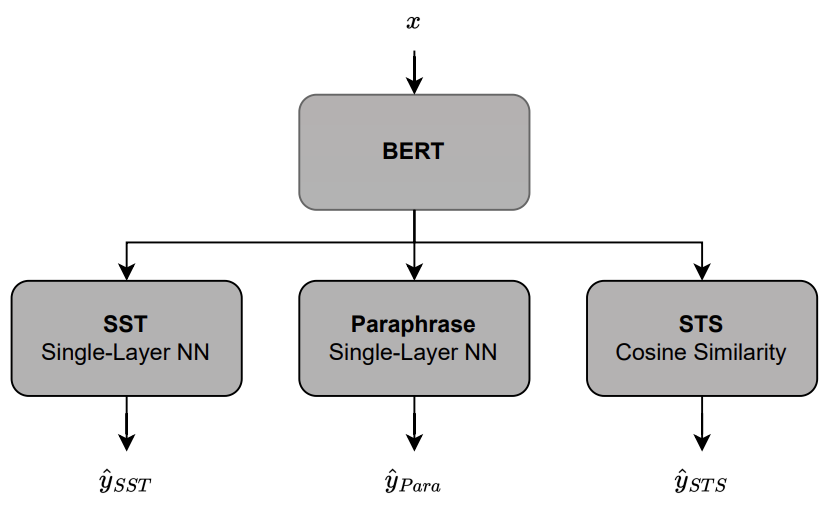
\includegraphics[width=0.9\textwidth,valign=t]{writeup/round-robin.png}
        \footnotesize
        \caption{Round-robin architecture.}
        \label{fig: vacc-rate}
    \end{subfigure}
    \begin{subfigure}[H]{0.49\textwidth}
    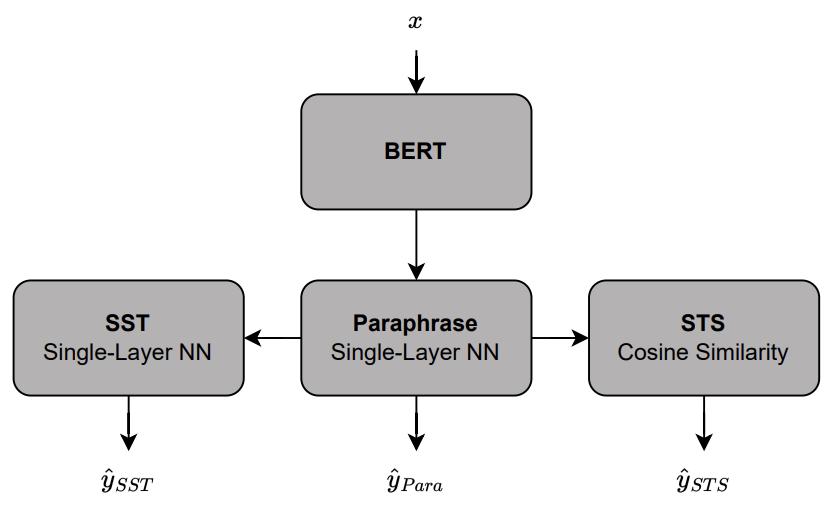
\includegraphics[width=0.9\textwidth,valign=t]{writeup/add-pretrain.png}
        \footnotesize
        \caption{Additional pre-train architecture.}
        \label{fig: sia-eff}
    \end{subfigure}
    \caption{Network architectures for our round-robin (a) and additional pre-training (b) approaches. Both approaches take as input textual data $x$, feed this through a pre-trained BERT model, and then focus on specific tasks. Note that (a) may take different-sized batches $x_B$ of data per task.}
    \label{fig: round-robin-arch}
\end{figure}
\vspace{-0.2cm}
\subsection{Rich Relational Layer Combining Similar Tasks}
 In addition to fully capturing the richness of our data, we further adapt our model to handle relations across tasks. That is, when tasks are similar, overall learning may benefit from combining the signals in these tasks' data. To do this, we propose using a combined relational layer between similar tasks before task-specific fine-tuning, much like MT-DNN \cite{MTL}. We hypothesize this is especially helpful when data for some of the combined tasks is scarce. Essentially, this idea applies transfer learning like we do with minBERT, but now to a more specialized setting of similar tasks.
 
 Of the three downstream tasks we use for evaluation, we note that the paraphrase and semantic textual similarity tasks are closely related; both evaluate the similarity of sentence pairs (albeit on different scales). In addition, the STS dataset is much smaller than the Quora dataset. By funneling these two datasets through a shared layer (with LeakyReLU nonlinearity) before diverging into task-specific learning, we hope to exploit the richness of the paraphrase data to enhance STS learning. Although such a relational layer may already be useful in the equally-weighted batch setting, we focus on the interleaved round-robin approach, i.e., using as much of the paraphrase data to boost STS as possible. Note that such a shared layer, which maps embedding pairs to a single hidden layer embedding, does not allow us to use cosine similarity for STS anymore. Instead, we pass the scaled Hadamard product $\frac{h_u \odot h_v}{||h_u||_2 ||h_v||_2 + \epsilon}$ between paired embeddings $h_u$ and $h_v$ as a feature to the relational layer (summing this feature exactly returns cosine similarity). Figure \ref{fig: rich-rel-fig} visualizes this rich relational architecture.

 \begin{figure}[h]
    \centering
    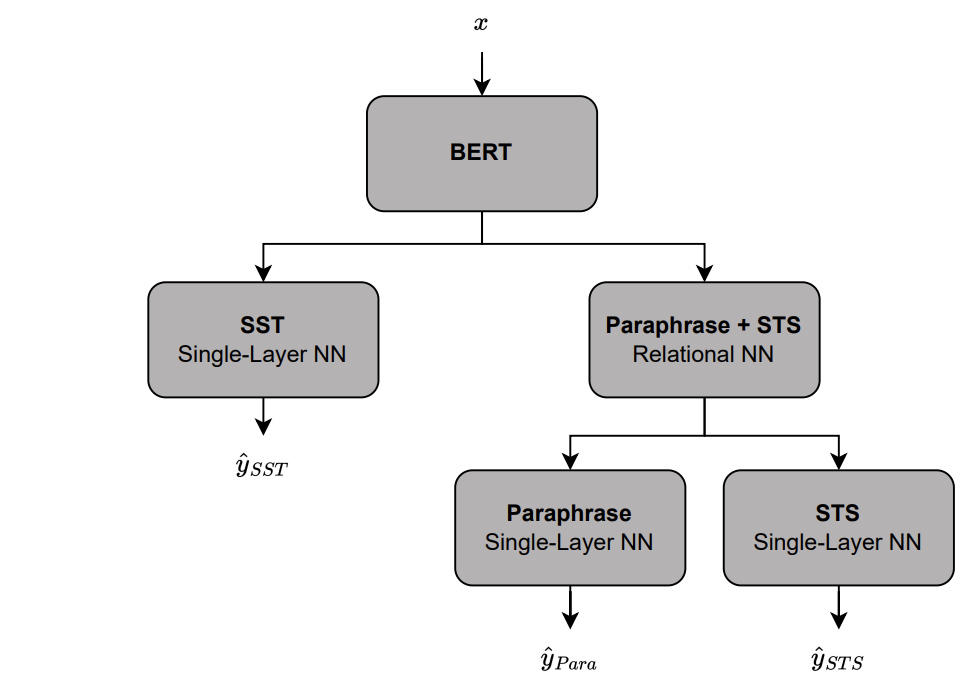
\includegraphics[width=0.49\textwidth]{writeup/rich-rel.png}
    \caption{Network architecture for the rich relational approach. The network takes as input textual data $x$, feeds this through BERT, and then splits into groups of similar tasks for fine-tuning.}
    \label{fig: rich-rel-fig}
\end{figure}

\section{Experiments}
\label{sec: experiments}
%In this section we discuss datasets, evaluation method, experiments performed and results so far.

% \textbf{Data}: Describe the dataset(s) you are using along with references. Make sure the task associated with the dataset is clearly described.
\subsection{Datasets} 
Our default minBERT model is pre-trained using two unsupervised tasks on Wikipedia articles: masked language modeling and next sentence prediction. For fine-tuning on downstream prediction tasks, we use the \textit{Stanford Sentiment Treebank} (SST), \textit{Quora}, and \textit{SemEval STS Benchmark} (STS) datasets. The SST dataset consists of 11,855 single sentence reviews, where a review is labelled categorically \{negative, somewhat negative, neutral, somewhat positive, positive\}. The Quora dataset consists of 400,000 question pairs with binary labels (true if one question is paraphrasing the other). The STS dataset consists of 8,628 different sentence pairs, each given a continuous score from 0 (unrelated) to 5 (equivalent meaning). In addition, for baseline evaluation, we use the \emph{CFIMBD} dataset, which contains 2,434 movie reviews, labeled as either positive or negative. Our datasets require some minimal pre-processing, including tokenizing sentence strings, lower-casing word tokens, standardizing punctuation tokens, and padding sentences to enable matrix multiplication.
 %For fine-tuning and evaluating our model on downstream prediction tasks, we use the Stanford Sentiment Treebank, Quora Dataset, and SemEval STS Benchmark Dataset. The \emph{Stanford Sentiment Treebank} (SST) dataset consists of 11,855 single sentence reviews, where a review is labelled categorically \{negative, somewhat negative, neutral, somewhat positive, positive\}. The \emph{Quora Dataset} (Quora) consists of 400,000 question pairs with binary labels (true if one question is paraphrasing the other). And, finally, the \emph{SemEval STS Benchmark Dataset} (STS) consists of 8,628 different sentence pairs, with each given a score from 0 (unrelated) to 5 (equivalent meaning). 
% Our datasets require some minimal pre-processing, including tokenizing sentence strings, lower-casing word tokens, standardizing punctuation tokens, and padding sentences to enable matrix multiplication.

% \item \textbf{Experimental details}: Please explain how you ran your experiments (e.g. model configurations, learning rate, training time, etc.).
\subsection{Experimental Details} 
All experiments share some general settings; we run 10 epochs with a fine-tune learning rate of 1e-5 and a hidden-layer dropout probability of 0.3. For our pretrain default minBERT model, we use a learning rate of 1e-3. When memory allows us to, we set our batch size to be 64.

\textbf{Regularization of Loss and Optimizer Step [smart]} The hyperparameter values specific to our SMART \cite{smart} implementation are $\lambda = 5$, $\epsilon = 1e-5$, $\sigma = 1e-5$, $\beta = 0.995$, $\mu = 1$, and $\eta = 1e-3$. Due to memory usage, we reduce our batch size to 16 rather than 64. We experimented with $\lambda$ to ensure that our adjustments would be applied at the right order of magnitude.

\textbf{Round-Robin Multitask Fine-Tuning [rrobin]} For equally-weighted round-robin, we fix batch size of 64 across all datasets and run \texttt{floor(len(sts\_train\_data) / args.batch\_size)} iterations per epoch. For round-robin with additional pretraining (rrobin-pre), we set batch size separately for the pretrain and round-robin portions. By default both are set to 64, but we ratchet down to 16 if running model with SMART. For interleaved round-robin (rrobin-full), we fix the number of iterations per epoch and correspondingly adapt the batch size per dataset. Given a maximum batch size of 64, set for the paraphrase data, we infer the batch sizes of SST and STS to be 3 and 2 respectively.

\textbf{Rich Relational Layer Combining Similar Tasks [rlayer]} The rich relational layer approach follows the same parametrizations as (interleaved) round-robin. That is, when equally weighting all datasets, we can use a batch size of 64, while we resort to smaller adjusted batch sizes for SST and STS when using all paraphrase data to be put through the relational layer.

% \item \textbf{Results}: Report the quantitative results that you have so far. Use a table or plot to compare multiple results and compare against your baselines.

\subsection{Results}
% \item \textbf{Evaluation method}: Describe the evaluation metric(s) you used, plus any other details necessary to understand your evaluation.
To evaluate the different models, we use accuracy for the sentiment analysis and paraphrase detection tasks, and pearson correlation for STS. We note that the SST dataset forms a multi-class classification task, while the paraphrase detection and CFIMDB labels are binary. 
\vspace{-0.4cm}
\begin{table}[h]
\footnotesize
\centering
\caption{\textit{Dev accuracy of baseline BERT models (pretrain and fine-tune) vs. benchmarks for single-task classifier and runtimes per training epoch on a Google Colab GPU.}}
\begin{tabular}{|l|ccc|ccc|}
\hline
  & \multicolumn{3}{c|}{\textbf{Sentiment (SST)}} & \multicolumn{3}{c|}{\textbf{Sentiment (CFIMDB)}} \\ \hline
\textbf{Model type}       & Accuracy       & Benchmark & Runtime (s)          & Accuracy        & Benchmark & Runtime (s)           \\ \hline
Pretrain default & 0.393           & 0.390 (0.007) & 30    & 0.788            & 0.780 (0.002)  & 45     \\
Fine-tune default & 0.522           & 0.515 (0.004) & 120    & 0.963            & 0.966 (0.007) & 150      \\ \hline
\end{tabular}
\label{tab: single}
\end{table}
% Although Table \ref{tab: single} is interesting from a single-task transfer learning perspective, we are, as discussed in Section \ref{sec: approach}, mostly concerned with multitask learning. 

In Table \ref{tab: single}, we report the dev set performance of our baseline pre-trained (min)BERT and fine-tuned models for sentiment classification alongside benchmarks from the project handout. Our results are all close to the benchmarks, which gives us confidence in the `correctness' of our implementation. The pre-trained BERT model clearly performs much better than random, indicating that its transfer learning is somewhat effective. However, fine-tuning drastically improves classification accuracy.

\vspace{-0.2cm}
\begin{table}[h]
\footnotesize
\centering
\caption{\textit{Dev set accuracies of single- and multitask models on three fine-tune tasks. The models are divided into three groups; (i) single-task approaches, (ii) small-scale (equally-weighted batches) approaches, and (iii) large-scale rich (relational) approaches. The best model for each task is bolded. Runtimes are given in seconds per training epoch on an AWS EC2 instance.}}
\begin{tabular}{|l|cccc|} \hline
& \multicolumn{1}{c}{\textbf{Sentiment (SST)}} & \multicolumn{1}{c}{\textbf{Paraphrase (Quora)}} & \multicolumn{1}{c}{\textbf{Similarity (STS)}} &  \\ \hline
\textbf{Model type} & Accuracy & Accuracy & Correlation & Runtime (s) \\ \hline
Pretrain default      & 0.396         & 0.380            & 0.019 & 9          \\
Fine-tune default      & 0.525        & 0.522           & 0.240 &  25         \\ 
Fine-tune smart        & 0.520             & 0.501           & 0.382 & 161          \\ \hdashline
Fine-tune rrobin       & 0.524            & 0.726            & 0.583   & 67        \\
Fine-tune rrobin+smart & \textbf{0.532}              & 0.741            & 0.680 & 464          \\ \hdashline
Fine-tune rrobin-pre+smart & 0.519          & 0.851           & 0.690 & 3,037         \\
Fine-tune rrobin-full & 0.498          & 0.863           & 0.762 & 1,420         \\ 
Fine-tune rrobin-full+smart & 0.485          & 0.850           & 0.714 & 4,549         \\
Fine-tune rrobin-full+rlayer & 0.501     & \textbf{0.867}         & \textbf{0.802}    & 1,550                 \\ \hline
\end{tabular}
\label{tab: multi}
\end{table}
% \vspace{-0.2cm}

Table \ref{tab: multi} gives the dev performance for all proposed model approaches on the SST, Quora, and STS tasks. We include three non-multitask models; the baseline models from Table \ref{tab: single} (i.e., BERT and fine-tuned SST) and an SST-fine-tuned model with SMART. Furthermore, we evaluate various multitask learning approaches combining SMART, round-robin, and the rich relational layer model.  

From Table \ref{tab: multi}, we can see that SMART performs best out of the single-task models, achieving the highest STS score. However, unsurprisingly, all multitask models easily beat these single-task baselines in terms of paraphrase and STS scores. Out of the multitask models that only use a limited portion of the available data (fine-tune rrobin, fine-tune rrobin+smart), the SMART implementation again performs best, especially in terms of STS score. It seems that, using a limited amount of data, this task is particularly prone to overfitting when trained without regularization. When making use of the entire Quora data, we can see that paraphrase accuracy is significantly boosted, reaching values over 85\%. In this setting, it seems that the added value of SMART vanishes. Namely, STS scores for the non-SMART models exceed those from SMART models. 

The best model overall is the rich relational interleaved round-robin model, which achieves test set performances of 0.503 (SST), 0.865 (paraphrase), and 0.789 (STS). This model stands out in its STS score, which confirms our hypothesis that capturing correlations between paraphrase and STS data through a shared layer can boost similar tasks' performance. In terms of runtime, SMART is most costly, especially when used in combination with richer data.

% (*) As a sense check, we verify that default pretrain and finetune accuracies approximately match results from single-task classifier.

% \begin{center}
% \begin{tabular}{||c |c : c|c : c|c : c||}
%     \hline
%         Model & \multicolumn{2}{ c |}{Sentiment (accuracy)} & \multicolumn{2}{ c |}{Paraphrase (accuracy)} & \multicolumn{2}{ c ||}{Similarity (correlation)} \\
%     \hline \hline 
%         pre-baseline & .78 & .78 & .78 & .78  &  .78    & .78 \\ 
%     \hline
%         finetune-baseline  & .78  & .78  & .78  & .78  &  .78 &  .78  \\
%     \hline
%         SMART & .78  &  .78  &  .78 &  .78  &  .78   &  .78 \\
%     \hline
% \end{tabular}
% \end{center}


\section{Analysis}
\label{sec: analysis}

\subsection{Qualitative Deepdive}
\label{sec: deepdive}
%After the milestone submission, we invested time to interrogate the results of our models and better understand the datasets and prediction tasks. Below, we briefly discuss some important observations. 

\textbf{Sentiment Classification (SST).} The distribution of SST classes is not uniform, with classes 0 and 4 (strong negative and positive) being less represented at 12.6\% and 14.9\%, respectively, and classes 1-3 being more represented at 26.2\%, 20.8\% and 25.3\%, respectively. Theoretically, we would expect these middle classes to be more difficult to predict, since their conveyed sentiment is less straightforward. For example, when reading the sentence "It's a lovely film with lovely performances by Buy and Accorsi", we could very well assess this to be a strong positive (class 4), but the actual label is somewhat positive (class 3). It turns out that the SST multi-class classification task is hard; the highest reported accuracy is around 59\% \cite{heinsen2022algorithm}. To identify how this class difficulty affects our predictions, Table \ref{tab: class-sst} provides precision, recall, and $F_1$-scores, from which we find that the "neutral" class is most difficult to predict, and the model is biased to predicting the most frequent classes.

\begin{SCtable}[][h]
\footnotesize
% \centering
\begin{tabular}{|l|ccc|} \hline
Class             & Precision & Recall & F1 score \\ \hline
negative          & 0.57      & 0.27   & 0.36     \\
somewhat negative & 0.51      & 0.69   & 0.58     \\
neutral           & 0.38      & 0.20   & 0.26     \\
somewhat positive & 0.48      & 0.79   & 0.60     \\
positive          & 0.74      & 0.30   & 0.43     \\ \hline
\end{tabular}
\caption{\textit{Precision, recall, and $F_1$-scores for all SST class labels corresponding with our top model.}}
\label{tab: class-sst}
\end{SCtable}
% \vspace{-0.2cm}

\textbf{Paraphrase Identification (Quora).} Our early (small) models produced much worse dev results than train results. To sanity check this result, we analyzed the ratios of true vs. false paraphrase pairs in the train and test datasets. These turned out to be well-balanced:  37\% : 63\% and 38\% : 62\%, respectively. This gave us confidence that we were dealing with an overfitting issue and prompted us to focus on implementing regularization techniques. 

\textbf{Semantic Textual Similarity (STS).} The difficulty we faced with respect to STS early on was working with the distribution of its data and combining this with choosing our loss function. We tried various methods, such as a linear layer, but found that the multimodal nature of the data distribution (see Figure \ref{fig: true-dist}) made for difficult prediction-label alignment. We suspect this multimodality, which occurs around whole integers, is mostly due to labeling bias; people might prefer rounding labels to whole numbers. Following literature, we found that cosine similarity led to relatively decent correlation scores and we adjusted our rich relational architecture to incorporate a vectorized form of cosine similarity between embeddings as a feature. Still, when we look at the distribution of our embeddings (see Figure \ref{fig: skewed-pred}), this distribution is relatively skewed. An interesting area for future research would be to try and handle the distribution of STS labels more adequately.
\vspace{-0.3cm}
\begin{figure}[h]
    \centering
    \begin{subfigure}[b]{0.49\linewidth}
    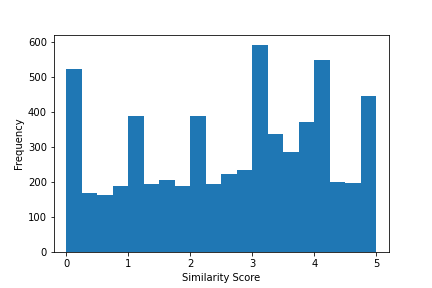
\includegraphics[width=\linewidth]{true_sts.png}
        \caption{True STS label distribution.}
        \label{fig: true-dist}
    \end{subfigure}
    \begin{subfigure}[b]{0.49\linewidth}
        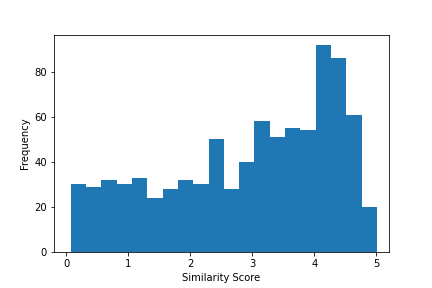
\includegraphics[width=\linewidth]{pred_sts.png}
        \caption{Predicted STS label distribution.}
        \label{fig: skewed-pred}
    \end{subfigure}
    \caption{Side-by-side comparison of true vs. predicted STS distributions.}
    \label{fig:ps3q3e}
\end{figure}
\vspace{-0.2cm}

\textbf{Sentence Pairs.} Last, one of our major conceptual breakthroughs came from recognizing the usefulness of the paraphrase dataset for enriching our model to predicting textual similarity. Both datasets tackle the task of evaluating the similarity of a pair of sentences. This leads to large correlations between the textual information contained in the two datasets, which, in combination with the large size differences, makes for a high combination potential. While we do not expect perfect correlations, this notion does lead us to hypothesize that pooling learning weights across these tasks during fine-tuning can be beneficial. An example of clearly similar sentence pairs is given by
\begin{align*}
    &\text{STS: \textit{How do you know what is right and wrong?} \textbf{vs.} \textit{How do you know which story is the right one?}} \\
    &\text{PAR: \textit{How are right and wrong defined? And why} \textbf{vs.} \textit{What is right and what is wrong?}}
\end{align*}

% Add in paragraph about why adding SMART to small dataset MTL implementation is effective.
\subsection{Experiment Findings} 
% \vspace{-0.2cm}
The following paragraphs detail the interpretation of our experiment results as well as some successes and failures. Firstly, we note that, from Table \ref{tab: single}, applying fine-tuning to BERT weights clearly allows us to boost performance on a single downstream task. However, such a single-task fine-tune model does not generalize well to other prediction tasks, which we observed from looking at the single-task approaches in Table \ref{tab: multi}. This naturally paved the way for us to consider multitask learning approaches.   

Compared to a single-task model trained on SST data, we found that an equally-weighted round-robin approach (fine-tune rrobin in Table \ref{tab: multi}) provided a meaningful boost to our results. The core idea here was to avoid destroying performance on sentiment analysis by introducing fine-tuning for other tasks in a balanced way, i.e., use the same amount of training data for each task for each fine-tuning iteration. However, in doing so, we encountered overfitting.  

This led us to implementing SMART. The efficacy of SMART relies on preserving structure learned from pre-training and preventing possible roughness induced from a fine-tuning dataset. This effect is pronounced when the fine-tuning dataset is small or ill-balanced. Areas of the feature space that are sparsely covered in such a dataset will tend to create sharp decision boundaries that may not be generalizable, and hence perform poorly on out-of-sample tests. Our results seem to confirm this belief. By adding SMART to our default fine-tune model, we improve STS by around $14\%$, while adding SMART to our round-robin fine-tune model (fine-tune rrobin+smart) causes an increase of around $17\%$ in the STS score. All the while, the other two tasks' performance remains stable. This result seems natural since we are operating in a low-data environment, where the number of unique training examples is constrained by the smallest size of the three tasks. 
% In this case, SMART can enforce additional structure via smoothness that reduces the need for additional data points, thus making the decision boundaries and solution surface better able to predict out-of-sample data points.

%We obtain an improved result when combining the round-robin extension with SMART (rrobin+smart), attaining better scores for all three tasks than either of the individual extensions.
 %With more observations, the model should be able to recover this kind of behaviour on its own, but as the fine-tuning data size decreases, this kind of regularization seems to become important.  
Since our default and equally-weighted round-robin models do not make use of all available data, this led us to focus on learning in a richer environment. Firstly, we tried incorporating the full Quora dataset by using it in an additional "pretraining" layer and then proceeding with multitask learning (rrobin-pre+smart). As Table \ref{tab: multi} shows, this provided a meaningful increase in performance beyond our milestone results for both the paraphrase and semantic textual similarity tasks. Thus, we learned that the Quora dataset, while obviously relevant to our paraphrase task, was also helpful for textual similarity. This motivated us to test the hypothesis that the advantage of introducing more data was greater than the potential risk of imbalanced fine-tuning. We tested a more sophisticated multitask method that interleaved the larger Quora dataset into fine-tuning by using variable batch sizes for each dataset (rrobin-full). As hoped, this further boosted performance, especially for STS.

Interestingly, Table \ref{tab: multi} shows that adding SMART regularization to this model (rrobin-full+smart) does not improve performance. This could be explained by the fact that the incremental benefits of regularization decrease with the size of data used and regularization may even restrict learning too much in this setting. It is also very well possible that the need for a lower batch size in rich data SMART settings causes too much learning variance.   

The improvement of STS scores when including the full Quora dataset as well as the sentence pair deepdive in Section \ref{sec: deepdive} imply some kind of correlation between the paraphrase and STS tasks. To make use of this correlation, we designed a rich and relational architecture (Figure \ref{fig: rich-rel-fig}) that uses all data while doing shared learning on similar tasks (rrobin-full+rlayer). This model proved to be our best, with paraphrase and STS scores both exceeding 0.8. Note, for all rich-data models, SST accuracy slightly dropped. This is likely caused by the added Quora data being irrelevant to or disrupting the sentiment task. Still, the decrease in SST accuracy is small relative to the gain in paraphrase and STS scores, which leads us to believe that SST is somewhat `orthogonal' to the other tasks. 
 
This notion of correlation and orthogonality prompted us to design our training steps. Namely, we started off by adding loss functions for the three prediction tasks and performing a single backward and optimization step for this combined loss in each training iteration. However, we found that taking sequential separate steps per prediction tasks improved performance. This can be explained by the gradient updates for the three tasks to be either very much aligned (STS and paraphrase) or relatively orthogonal (SST). In addition, this way, we take more optimization steps and do not face scale issues when adding up losses of totally different orders of magnitude.
\vspace{-0.2cm}
\section{Conclusion}
\label{sec: conclusion}
\vspace{-0.2cm}
In this project, we investigated the performance of a pre-trained and fine-tuned BERT model on three downstream prediction tasks when we include (1) regularization in our fine-tuning loss function and parameter gradient step (SMART by Jiang et al. \cite{smart}), (2) multitask learning with task-specific datasets, and (3) rich relational layers that exploit similarity between tasks. We found that our best model combines multitask learning using varying batch sizes with a rich relational layer between correlated tasks. While including SMART regularization was helpful for smaller fine-tuning datasets with larger batch sizes, we found its effects were washed out when we incorporated richer data.

In terms of next steps, we would like to explore (1) data transformations that allow for continuous multimodal distributions (for semantic similarity); (2) more advanced pretrained encoder models such as RoBERTa or ALBERT; and (3) incorporating CFIMDB into our multitask fine-tuning routine paired with SST through a rich relational layer.


\newpage
\textit{Contributions: Quinn owned development of the SMART regularization implementation. Julian owned development of the round-robin multitask learning. Thomas owned development of our rich relational layer as well as the qualitative deepdive. Everyone contributed to the default model setup, running experiments on AWS server, and brainstorming design choices.}

\bibliographystyle{unsrt}
\bibliography{references}

\newpage
\appendix
\section{SMART: Adversarial Loss Calculation}
\begin{algorithm}[h]
\KwData{$\hat{f}$: model, $\{x_{i}\}_{1}^{Q}$: model embeddings, $\{z_{j}\}_{1}^{B}$: batch inputs, $\sigma^{2}$: variance of noise, $\eta = 10^{-3}$: learning rate for adversarial update, $\epsilon = 10^{-5}$: max perturbation.}
\Begin{
    $\hat{f}$ set to eval mode \\
    $y_{j} \longleftarrow \hat{f}(z_{j}, x)$ \\
    \For{$ x_{i} \in \mathcal{Q}$}{
        $\Tilde{x}_{i} \longleftarrow x_{i} + \nu_{i}$    with $\nu_{i} \sim \mathcal{N}(\mathbf{0}, \sigma^{2} \mathbf{I})$
    } 
    \For{$ y_{j} \in \mathcal{B}$}{
        $\Tilde{h}_{j} \longleftarrow \nabla_{\tilde{x}} l_{s}(y, \hat{f}(z_{j}, x))$
    }
    $\Tilde{g}_{i} \longleftarrow \left(\frac{1}{|\mathcal{B}|} \sum_{i} \Tilde{h}_{j} \right)\left( \lVert    \frac{1}{|\mathcal{B}|} \sum_{i} \Tilde{h}_{j} \rVert_{\infty}\right)^{-1}$ \\
    \For{$x_{i} \in \mathcal{Q}$}{
        $\Tilde{x}_{i} \longleftarrow \mathcal{P}_{\lVert \Tilde{x}_{i} + \eta \Tilde{g}_{i} - x_{i}\rVert \leq \epsilon} \left( \Tilde{x}_{i} + \eta \Tilde{g}_{i} \right)$
    }
    $y^{\text{adv}}_{j} \longleftarrow \hat{f}(z_{j}, \Tilde{x})$ \\
    $\mathcal{L}_{\text{adv}, \text{classification}} \longleftarrow \frac{1}{|\mathcal{B}|} \sum_{j \in \mathcal{B}} \mathcal{D}_{KL}( y_{j} || y^{\text{adv}}_{j}) + \mathcal{D}_{KL}( y^{\text{adv}}_{j} || y_{j})$ \\
    $\mathcal{L}_{\text{adv}, \text{regression}} \longleftarrow \frac{1}{| \mathcal{B} |} \sum_{j \in \mathcal{B}} \lVert y_{j} - y^{\text{adv}}_{j} \rVert^{2}$ \\
    $\hat{f}$ set to train mode
}
\caption{SMART: Adversarial Loss Calculation}
\label{alg: smart-adv}
\end{algorithm}

\end{document}